\documentclass{beamer}
\usepackage{graphicx} % Required for inserting images
\usepackage{quiver}
\usepackage{adjustbox}
\usepackage{bussproofs}
\usepackage{wasysym}
\usepackage[normalem]{ulem}
\usepackage{marvosym}
\usepackage{stmaryrd}

\usepackage{amsmath}
\usepackage{amssymb}
\newcommand{\cat}[1]{\mathsf{#1}}
\newcommand{\typesetcategory}[1]{\cat{#1}}
\newcommand{\C}{\mathcal C}
\newcommand{\Set}{\mathrm{Set}}
\newcommand{\Th}{\mathtt{Th}}
\newcommand{\QTh}{\mathtt{QTh}}
\DeclareMathOperator{\ar}{ar}

\usepackage{xcolor}

\setbeamertemplate{navigation symbols}{}


\makeatletter
\newcommand{\Pause}[1][]{\unless\ifmeasuring@\relax
\pause[#1]%
\fi}
\makeatother

\usetheme{Madrid}
\usecolortheme{beaver}

\title{Algebraic Reasoning for Nondeterministic and Probabilistic Programs}
\subtitle{\small ``The Theory of Traces for Systems with
Nondeterminism, Probability, and Termination'' \\ by
Bonchi, Sokolova, Vignudelli\\ ``Combining Nondeterminism, Probability, and Termination: Equational and Metric Reasoning'' \\ by Mio, Sarkis, Vignudelli}
\author{Anny Beatriz Azevedo and Augustin Albert}
\date{June 17 2026}

\begin{document}

\maketitle

\part{Presentation of a Monad}\frame{\partpage}

\begin{frame}{Effectful Automata}

\begin{block}{Coalgebra}
Let $F : \mathsf{C} \to \mathsf{C}$ be an endofunctor. An \textbf{$F$-coalgebra} is an object $X\in \operatorname{Ob}(\mathsf{C}) $ along with a morphism $\sigma: X \to FX \in \operatorname{Mor}(\mathsf{C})$.
\end{block}

\pause

\begin{block}{Monad}
A \textbf{monad} is a functor $M$ along with natural transformations $\eta_X:X \to MX $ and $\mu_X: M^2X \to X$ such that certain diagrams commutes.
\end{block}
\pause

\begin{block}{Automata with effects}
Let $M$ be a $\mathsf{Set}$-monad and $O, A$ be
sets. An \textbf{$A$-automaton with $M$-effects and observations in $O$} is a coalgebra $S \to O \times (MS)^A$
\end{block}

\pause

\begin{example}
    \begin{itemize}
        \item A deterministic automaton is a coalgebra $S \to 2 \times S^A$.
        \item A nondeterministic automaton is a coalgebra $S \to 2 \times (\mathcal P S)^A$.
    \end{itemize}
\end{example}
\end{frame}

\begin{frame}{Monads for Nondeterminism or Probability}
\begin{block}{Nondeterminism}
$\mathcal P$ is the  \textbf{powerset} $\mathsf{Set}$-monad, mapping a set $S$ to the set of subsets of $S$. 
\end{block}\pause

\begin{block}{Probability}
$\mathcal D$ is the \textbf{probability distribution} $\mathsf{Set}$-monad, mapping a set $S$ to the set of finitely supported probability distributions on $S$.
\end{block}
\pause

There is no monad distribution law between these two monads. Can we still compose them somewhat?
\end{frame}

\begin{frame}{The Monad $\mathcal C$ of Nondeterminism and Probability}

Recall the $\mathsf{Set}$-monad $(\C, \eta^\C, \mu^\C)$ of finitely generated, nonempty convex subsets of distributions. In particular:

$$\C X = \{S \subseteq \mathcal DX : S \neq \emptyset, \operatorname{conv}(S) = S, S \text{ is finitely generated} \}$$

% $$\text{with }\operatorname{conv}(S)=\left\{\sum p_i x_i : p_i\in [0,1],\sum p_i=1,x_i \in S\right\}$$
{
\centering

\pause

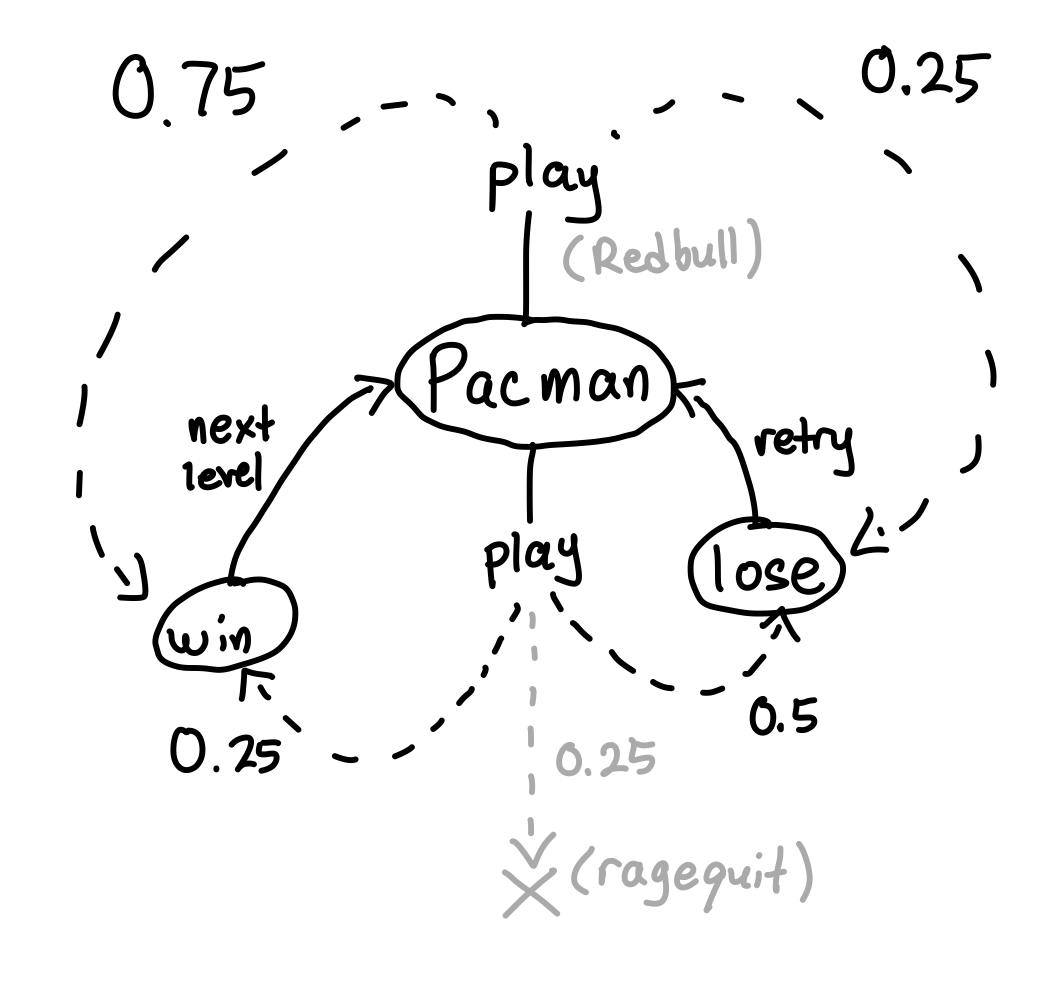
\includegraphics[width=.45\linewidth]{pacman.png}

}
\vspace{-.5\baselineskip}

Alyssa's Pacman game, using $O = 1 =\{*\}$ and the terminal state $\star$. %= \C1$ the free algebra of observations 

% No termination, so no subdistributions yet!
    
\end{frame}

\begin{frame}{Determinization of Effectful Automata}

\begin{block}{Determinization of Automata}
For all automata $S \to O \times (MS)^A$ and algebra $MO \to O$, its  \textbf{determinization} is a coalgebra $MS \to O \times (MS)^A$.
\end{block}

\pause

\begin{example}
    The determinization of a non deterministic automaton $S \to 2 \times (\mathcal P S)^A$ is a deterministic automaton $\mathcal P S \to 2 \times (\mathcal P S)^A$.
\end{example}

\pause

\begin{example}
    For \textbf{Pacman}, $\C O = 1 = O$, so the identity algebra suffices.
\end{example}

\pause 

Wouldn't it be nice if we could draw the determinization of the \textbf{Pacman} game?
\pause
That would require a nifty notation for the new determinized states, i.e., the elements of $\C S$\ldots

\end{frame}

\begin{frame}{Symbols...}
% Let $S$ be a finite set.
% \vspace{\baselineskip} 
% Recall that distribution are finitely supported !!
 \begin{block}{For $\mathcal D S$:}
\begin{itemize}
    \item For all $s \in S$, let $\mathbf s$ denote the distribution $\delta_s \in \mathcal D S$.  \pause
    \item For all $d_1, d_2 \in \mathcal D S$, $\alpha \in [0,1]$, let $d_1 +_\alpha d_2$ denote the distribution $\alpha \times d_1 + (1-\alpha) \times d_2 \in \mathcal D S$. \pause %: $$s \in S \mapsto \begin{cases}
        %\alpha \text{ if } s = s_1,\\
        %1- \alpha \text{ if } s = s_2,\\ 
        %0  \text{ otherwise}\end{cases}
    %$$
    \item[\MVRightarrow] We can write any distribution $d$ in $\mathcal D S$ as $d = \mathbf s_1 +_{\alpha_1} \cdots +_{\alpha_{n-1}} \mathbf s_n$. \pause
    \end{itemize}
    \end{block}
    
    \begin{block}{For $\C S$:}
    \begin{itemize}
    \item Elements of $\mathcal D S$ are regarded as elements of $\mathcal C S$: $\forall d \in \mathcal DS$, $\{d\} \in \mathcal CS$.\pause
    \item For all $d_1 \oplus d_2 \in \mathcal D S$, let $d_1 \oplus d_2$ denote the convex hull of $d_1$ and $d_2$ \pause
    \item[\MVRightarrow] We can write any $\varphi \in \C S$ as $x = (\mathbf s_{11} +_{\alpha_{11}} \cdots) \oplus \cdots \oplus (\mathbf s_{n1} +_{\alpha_{n1}} \cdots)$. \pause
    
\end{itemize}
\end{block}

All the elements of $\C S$ can be represented by a finite expression in the language $L(S) = S \cup \{ \overline \oplus \} \cup \{\overline +_\alpha\ \ | \ \alpha \in [0,1]\}$. We can denote our states using expressions in the language $L(S)$!

\end{frame}



\begin{frame}{...and Equations!}

All the elements of $\C S$ can be represented by a finite expression in the language $L(S) = S \cup \{ \overline \oplus \} \cup \{\overline +_\alpha\ \ | \ \alpha \in [0,1]\}$, \alert{ but this representation is not always unique!} \pause
    
   % \vspace{\baselineskip} \pause
    \begin{example}
         For all $s_1, s_2 \in S$ and $d_1, d_2, d_3 \in \mathcal D S$:

        \begin{itemize}
            \item $ s_1 +_\alpha  s_1 = s_1$
            \item $ s_1  +_\alpha  s_2 =  s_2 +_{(1-\alpha)}  s_1$
             \item $(d_1  \oplus d_2)  \oplus d_3 = d_1  \oplus (d_2  \oplus d_3)$ \pause
        \end{itemize}
    \end{example}
   

To ensure uniqueness, we need to quotient $L(S)$ by some equations\ldots \vspace{\baselineskip}\pause

\alert{Also, do all expressions represents elements of $\C S$?}\\ Consider for example $\varphi \oplus \psi$ for arbitrary $\varphi, \psi\in \C S$\ldots


\end{frame}

\begin{frame}{Presentations of a Monad}
In other words, we wish for a presentation of the monad $\C$:

\begin{block}{Presentation of a monad $M$}
    A \textbf{presentation} of $M$ is an algebraic theory $(\Sigma, E)$ such that $M$ is isomorphic to the term monad  \(T_{(\Sigma, E)}\) mapping sets of variables to \(\Sigma\)-terms modulo \(E\).
\end{block}

\pause 

\begin{block}{Lemma}
$(\Sigma, E)$ presents $M$ iff the Eilenberg-Moore category of \(M\)-algebras is concretely equivalent to the category of \textbf{models} of \((\Sigma, E)\).%: sets \(A\) equipped with operations interpreting the signature symbols that satisfy the axioms.
\end{block}

\pause

Presentations are nice!
\begin{itemize}
    \item Graphical representations of the determinization of an automaton
    \item Description of the structure required on $O$ to get an algebra $MO \to O$
    \item Equational reasonings for proving equivalences of programs\ldots
\end{itemize}

\end{frame}

\begin{frame}{A presentation for $\C$}


\(\mathcal{C}\) is presented by the theory \(\Th_{CS}\) of convex semilattices, with signature $\{ \oplus \} \cup \{+_\alpha\ \ | \ \alpha \in [0,1]\}$ and equations:
\[
\begin{aligned}
&\text{(A)} && x \oplus (y \oplus z) = (x \oplus y) \oplus z \\
&\text{(C)} && x \oplus y = y \oplus x \\
&\text{(I)} && x \oplus x = x \\
&\text{(A}_p\text{)} && (x +_q y) +_p z = x +_{pq} (y +_{\frac{1-q}{1-p}} z) \\
&\text{(C}_p\text{)} && x +_p y = y +_{1-p} x \\
&\text{(I}_p\text{)} && x +_p x = x \\
&\text{(D)} && x +_p (y \oplus z) = (x +_p y) \oplus (x +_p z)
\end{aligned}
\]\pause

\begin{itemize}
    \item[\MVRightarrow] For each element $\phi \in \mathcal C S$, there is a unique term $t$ in the language \(\Th_{CS}\) such that $\llbracket t \rrbracket = d$.
\end{itemize}
 
\end{frame}

\begin{frame}{Pictures, please!}

\begin{columns}
    \begin{column}{.34\linewidth}
         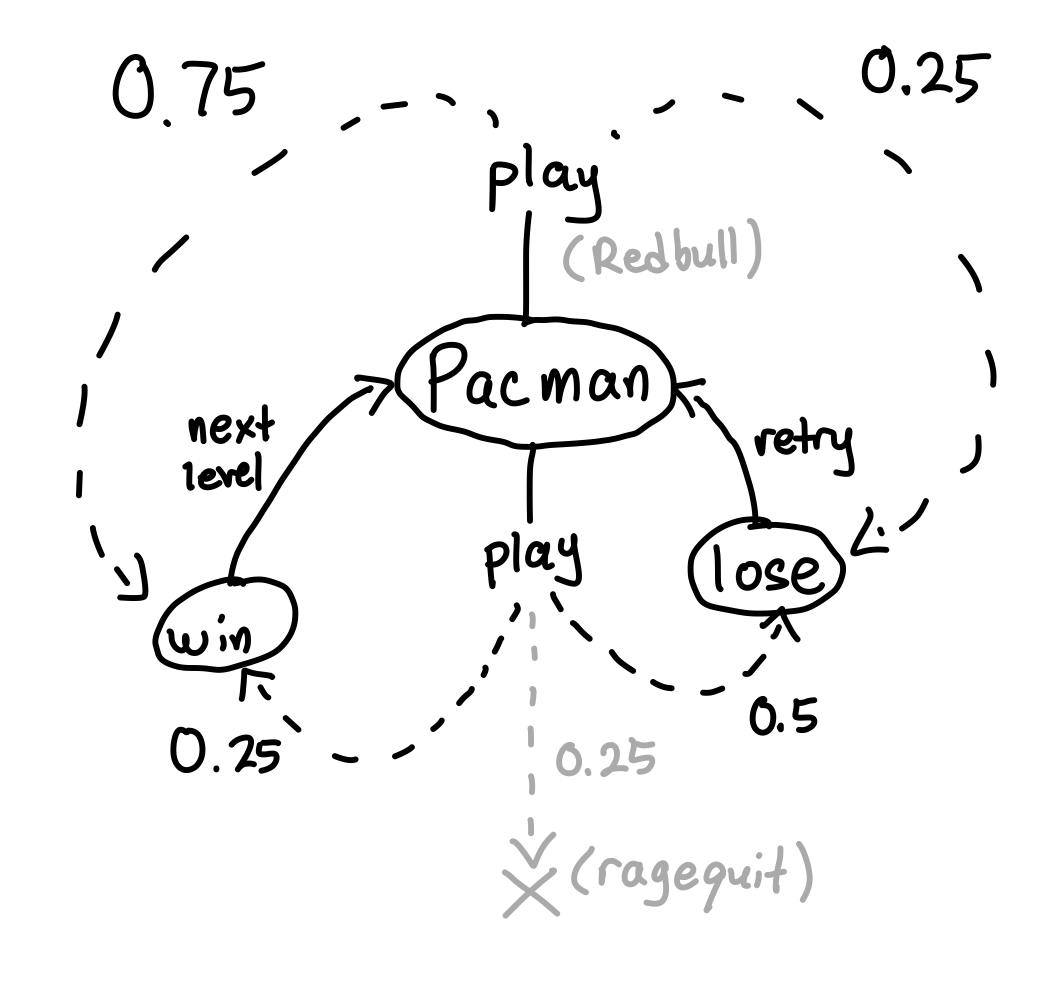
\includegraphics[width=\linewidth]{pacman.png}
    \end{column}
    \begin{column}{.65\linewidth}
We now know that $\mathtt{Pacman}$, $\mathtt{win} +_{3/4} \mathtt{lose}$, etc are the states of the determinization. \pause How to compute the transitions efficiently?
    \end{column}
\end{columns}
 \pause 
\vspace{-2\baselineskip}
 
 \begin{align*}
     &\mathtt{Pacman}\\ \Pause
    &\downarrow \mathtt{play}\\
    (\mathtt{win} +_{0.75} \mathtt{lose}) \oplus  &((\mathtt{win} +_{0.5} \star) +_{0.5} \mathtt{lose})\\ \Pause
    & \downarrow \mathtt{next\ level}\\
    (\mathtt{Pacman} +_{0.75} \star) \oplus  &((\mathtt{Pacman} +_{0.5} \star) +_{0.5} \star)\\ \Pause
    = (\mathtt{Pacman} +_{0.75} &\star) \oplus (\mathtt{Pacman} +_{0.25} \star)
 \end{align*}
   
    
\end{frame}

% \begin{frame}{Computing in Determinized Automata using Presentations}
%     TODO
% \end{frame}

% \begin{frame}{We did not modeled termination so good\ldots}

% Consider the following automaton with effects in $\C$, output set $O = 1$ and a hidden terminal state $\star$.

% TODO 

% \pause 

% Its determinization is  

% \begin{block}{Trace Equivalence in the Determinization}
% TODO
% \end{block}

% \begin{example}
%     TODO for pacman
% \end{example}
% \end{frame}

\part{Incorporating Termination}\frame{\partpage}


\begin{frame}{Termination}
\begin{itemize}
    \item In some systems, we need something to represent termination

    \pause

    \item In the Pacman example we add a symbol to represent ragequit
    \pause
    
    \item But how to add termination in general? \pause It depends
\end{itemize}
\end{frame}

\begin{frame}{Termination monad $+1$}
    $$\begin{array}{cccl}
 +1 \colon & \cat{Set} &\longrightarrow& \cat{Set} \\
    &X &\longmapsto&   X + 1
\end{array}$$
    \pause
    where $1 = \{\star\}$ and $+$ denotes coproduct in $\cat{Set}$, which is the disjoint union
    \pause
    $$f \colon X \to Y \longmapsto f+1 \colon X+1 \to Y+1$$ $$\begin{array}{cccl}
 f+1 \colon & X+1 &\longrightarrow& Y+1 \\
    & x &   \longmapsto &  \left\{ \begin{array}{ll}
    f(x) , & \text{if } x \in X\\
    \star , & \text{if } x = \star
\end{array} \right.
\end{array}$$
    \pause
    $\begin{array}{ccclcccl}
\eta \colon & X &\longrightarrow& X+1, ~~~~ &\mu \colon& (X+1)+1 &\longrightarrow& X+1 \\
            &x & \longmapsto &  x ~~~~ & &x   &\longmapsto&   \left\{ \begin{array}{ll}
     x, & \text{if } x \in X\\
    \star , & \text{if } x = \star 
\end{array} \right.
    \end{array}$
\end{frame}


\begin{frame}{Termination}
    \begin{itemize}
        \item We are going to use the monad $+1$ to add termination
    \pause 
    \item Semantically we have the obvious options $\C(X+1)$ or $\C(X) + 1$
    \pause
    \item Using presentation, we have more options
    \end{itemize}
    
\end{frame}

\begin{frame}{Using the presentation tool}

    \pause
    
    \begin{block}{Presenting M(+1)}
        Given a presentation $(\Sigma, E)$ for a monad $M$, the monad $M(+1)$ is presented by the theory $(\Sigma', E)$ where $\Sigma'$ is $\Sigma$ together with an extra constant $\star$.
    \end{block}
    \pause
    $$\mathcal{P}(X+1) \cong \mathcal{P}(X) \cup \{A \cup {\star} : A \in \mathcal{P}(X)\}$$
    $$\mathcal{P} \text{ and } \star~ \text{  closed for combining (union) elements}$$
    \pause
    $$\mathcal{D}(X+1) \cong \{\text{non-empty distributions}\} \cup \{\star\colon X \to [0,1], \star(x)=0\}$$
    $$\cup \{\text{non-empty subdistributions}\}$$
    $$\mathcal{D} \text{ and } \star ~\text{  closed for combining (weighted distributions) elements}$$
    
\end{frame}

\begin{frame}{A presentation for $\C(+1)$}
$$X \mapsto X+1 \mapsto \C(X+1)$$
\pause
\(\mathcal{C}(+1)\) is presented by the theory \(\Th^{\star}_{CS}\) of pointed convex semilattices, with signature $\{ \oplus \} \cup \{+_\alpha\ \ | \ \alpha \in [0,1]\} \cup \{\star\}$ and equations:
\pause
\[
\begin{aligned}
&\text{(A)} && x \oplus (y \oplus z) = (x \oplus y) \oplus z \\
&\text{(C)} && x \oplus y = y \oplus x \\
&\text{(I)} && x \oplus x = x \\
&\text{(A}_p\text{)} && (x +_q y) +_p z = x +_{pq} (y +_{\frac{1-q}{1-p}} z) \\
&\text{(C}_p\text{)} && x +_p y = y +_{1-p} x \\
&\text{(I}_p\text{)} && x +_p x = x \\
&\text{(D)} && x +_p (y \oplus z) = (x +_p y) \oplus (x +_p z)
\end{aligned}
\]
\end{frame}


\begin{frame}{Presentation for $(+1)\C$}
    Another way of adding termination is to give meaning to $\star$ by adding axioms involving it\\
    \pause
    
    %$$X \mapsto \C(X) \mapsto \C(X) + 1$$
    %\pause
    %Giving meaning to $*$ (kills operation $+_p$ with $*$, don't know yet the meaning of the bottom axiom)   
    $$(\bot) ~~~~x \oplus \star = x $$
    \pause
    $$(BH) ~~~~x +_p \star = \star$$
    \pause
    \begin{itemize}
        \item The first axiom doesn't change anything when dealing with $\oplus$
        \pause
        \item The second axiom kills operation $+_p$ with $\star$
        \pause
        \item The two of them together make $\star$ act \textit{outside} the monad: \pause \(\Th^{\star}_{CS} \cup \bot \cup BH\) is a presentation for $(+1)\C$
    \end{itemize}
\end{frame}

\begin{frame}{Which way is better?}
\pause
    \begin{figure}
        \centering
        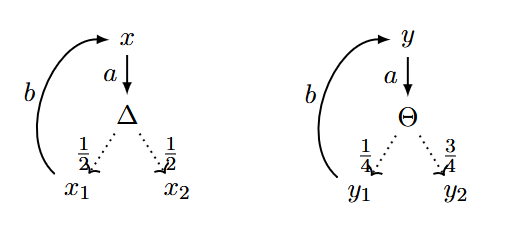
\includegraphics[width=0.5\linewidth]{images/im1.png}
    \end{figure}
    \pause
    $$x \downarrow_1 \xrightarrow{a} x_1 +_{\frac{1}{2}} x_2 \xrightarrow{b} x +_{\frac{1}{2}} \star \downarrow_{\frac{1}{2}}$$
    $$y \downarrow_1 \xrightarrow{a} y_1 +_{\frac{1}{4}} y_2 \xrightarrow{b} y +_{\frac{1}{4}} \star \downarrow_{\frac{1}{4}}$$
    \pause
    $$t^{\#}(x)(a)(b) = t^{\#}(x_1 +_{\frac{1}{2}} x_2)(b) = t(x_1)(b) +_{\frac{1}{2}} t(x_2)(b) = \star$$
    $$t^{\#}(y)(a)(b) = t^{\#}(y_1 +_{\frac{1}{4}} y_2)(b) = t(y_1)(b) +_{\frac{1}{4}} t(y_2)(b) = \star$$
\end{frame}

%\begin{frame}{Another way}
%    Example with $(+1)\C$, Segala systems
%\end{frame}

\begin{frame}{What if we look at an intermediate step?}
\pause
    \begin{itemize}
    \item We consider the theory  \(\Th^{\star}_{CS} \cup \bot = (x \oplus \star = x)\)\\
\pause
    \item We can prove that 
    $$x +_p y = (x+_p y) \oplus (\star +_p y) \oplus ((x+_q \star) +_p y)$$ 
    \end{itemize}
\end{frame}

\begin{frame}{What if we look at an intermediate step?}
    \begin{itemize}
    \item We consider the theory  \(\Th^{\star}_{CS} \cup \bot = (x \oplus \star = x)\)\\
    \item We can prove that 
    $$x +_p y = (x+_p y) \oplus \color{blue}{(\star +_p y)} \color{black}{\oplus} \color{red}{((x+_q \star) +_p y)}$$ \\
    which semantically means: 
    $$\color{blue}{\llbracket \star +_p y \rrbracket} \color{black}{\subseteq \llbracket x+_p y \rrbracket ~\text{and}~}\color{red}{\llbracket (x+_q \star) +_p y \rrbracket} \subseteq \color{black}{\llbracket x+_p y \rrbracket}$$\\
    \pause
    \item If $\varphi(x) ´= p$, it can be represented by $x +_p y$. If $\psi$ is a subdistribution defined as $\varphi$ except $\psi(x) < p$, we have two cases for $\psi(x)$:
    \begin{itemize}
        \item $\psi(x)=0$, represented by $\star +_p y$
        \item $\psi(x)$ is some value between $0$ and $p$, where we can always find a $q \in (0,1)$ st $\psi(x)=qp$, so $\psi$ can be represented by $(x +_q \star) +_p y$
    \end{itemize}
    \end{itemize}
\end{frame}

\begin{frame}{$\bot$-closed sets}
$$\llbracket \star +_p y \rrbracket \subseteq \llbracket x+_p y \rrbracket ~\text{and}~\llbracket (x+_q \star) +_p y \rrbracket \subseteq \llbracket x+_p y \rrbracket$$

    
    \pause
    \vspace{0.5cm}
    We have that if a convex set contains a subdistribution $\varphi$ with $\varphi(x)=p$, then it also contains any subdistribution $\psi$ defined as $\varphi$ except $\psi(x) < p$.
    \vspace{0.5cm}
    \pause
    \begin{block}{$\bot$-closed convex set}
    Let $X$ be a set and let $S \in \C(X + 1)$. We say that $S$ is \textbf{$\bot$-closed} if for all $\varphi \in S$ 
    $$\{\psi \in D(X + 1) : \forall x \in X, \psi(x) \leq \varphi(x)\} \subseteq S.$$
    \end{block}
    
\end{frame}

\begin{frame}{Monad $\C^{\downarrow}$}
We denote $\C^\downarrow(X)$ the sets $S \in \C(X+1)$ with for all $\varphi \in S$, $$\{\psi \in D(X + 1) : \forall x \in X, \psi(x) \leq \varphi(x)\} \subseteq S$$
\pause

\begin{block}{Monad $\C^{\downarrow}$} 

\begin{itemize}
    \item $X \longmapsto \C^{\downarrow}(X)$
    \item $f\colon X \to Y \longmapsto \C^{\downarrow}(f)\colon \C^{\downarrow}(X) \to \C^{\downarrow}(Y)$ defined as the restriction of $\C(f+1)$ to $\bot$-closed sets
    \item $\eta_{\C^{\downarrow}}(x) = \{p x + (1-p)\star : p \in [0,1]\}$
    \item $\mu_{\C^{\downarrow}}$ is defined as the restriction of $\mu_{\C(+1)}$ to $\bot$-closed sets.
\end{itemize}
\end{block}
\end{frame}

\part{Proving Equivalences of Processes using Presentations}\frame{\partpage}

\begin{frame}{A minimal Process Algebras}

Let $A$ be a set. Consider the language $\mathit{Proc}$ with terms:
\[
P ::= \operatorname{\overline{\star}} \mid P_1 \mathbin{\overline{\oplus}} P_2 \mid P_1 \mathbin{\overline{+}_p} P_2 \mid a.P, \quad a \in A
\]

\pause

\begin{itemize}
    \item $\operatorname{\overline{\star}}$ -- terminated process
    \item $a.P$ -- performs action $a$, then continues as $P$
    \item $\overline{\oplus}$ -- nondeterministic branching
    \item $\overline{+}_p$ -- probabilistic branching
\end{itemize}

\pause

\begin{example}
   $$ P_1 = a.(b.\operatorname{\overline{\star}} \overline +_{\frac12} \operatorname{\overline{\star}}) \mathbin{\overline{\oplus}} \operatorname{\overline{\star}}$$
   $$ P_2 = a^2.\operatorname{\overline{\star}}$$
   $$ P_3 = a.(a.\operatorname{\overline{\star}} \overline \oplus \operatorname{\overline{\star}})$$
   
\end{example}

\end{frame}

\begin{frame}{Continuations and Transition Semantics}
    Each process $P$ has a continuation $\tau(P) \in T_{\Th_{CS}^*}(Proc) \cong \mathcal{C}(Proc+1)$, written $P \rightarrowtail \tau(P)$, defined by induction:

\pause
\[
\frac{}{a.P \rightarrowtail P} \qquad
\frac{}{\operatorname{\overline{\star}} \rightarrowtail \star}
\]

\[
\frac{P_1 \rightarrowtail t_1 \quad P_2 \rightarrowtail t_2}
     {P_1 \mathbin{\overline{\oplus}} P_2 \rightarrowtail t_1 \oplus t_2} 
\qquad
\frac{P_1 \rightarrowtail t_1 \quad P_2 \rightarrowtail t_2}
     {P_1 \mathbin{\overline{+}_p} P_2 \rightarrowtail t_1 +_p t_2}
\]
\pause 
\vspace{\baselineskip}

This yields a coalgebra $Proc \to \mathcal{C}(Proc+1)$, i.e. a transition semantics. \pause We get another semantics by quotienting the continuation term by additional equations:

\begin{itemize}
    \item Quotienting by $(\bot)$ gives $Proc \to \mathcal{C}^\downarrow(Proc)$
    \item Quotienting by both $(\bot)$ and $(BH)$ gives $Proc \to \mathcal{C}(Proc)+1$
\end{itemize}

\end{frame}

\begin{frame}{The different transition semantics, concretely}
{$ P_1 = a.(b.\operatorname{\overline{\star}} +_{\frac12} \operatorname{\overline{\star}}) \mathbin{\overline{\oplus}} \operatorname{\overline{\star}}$}

    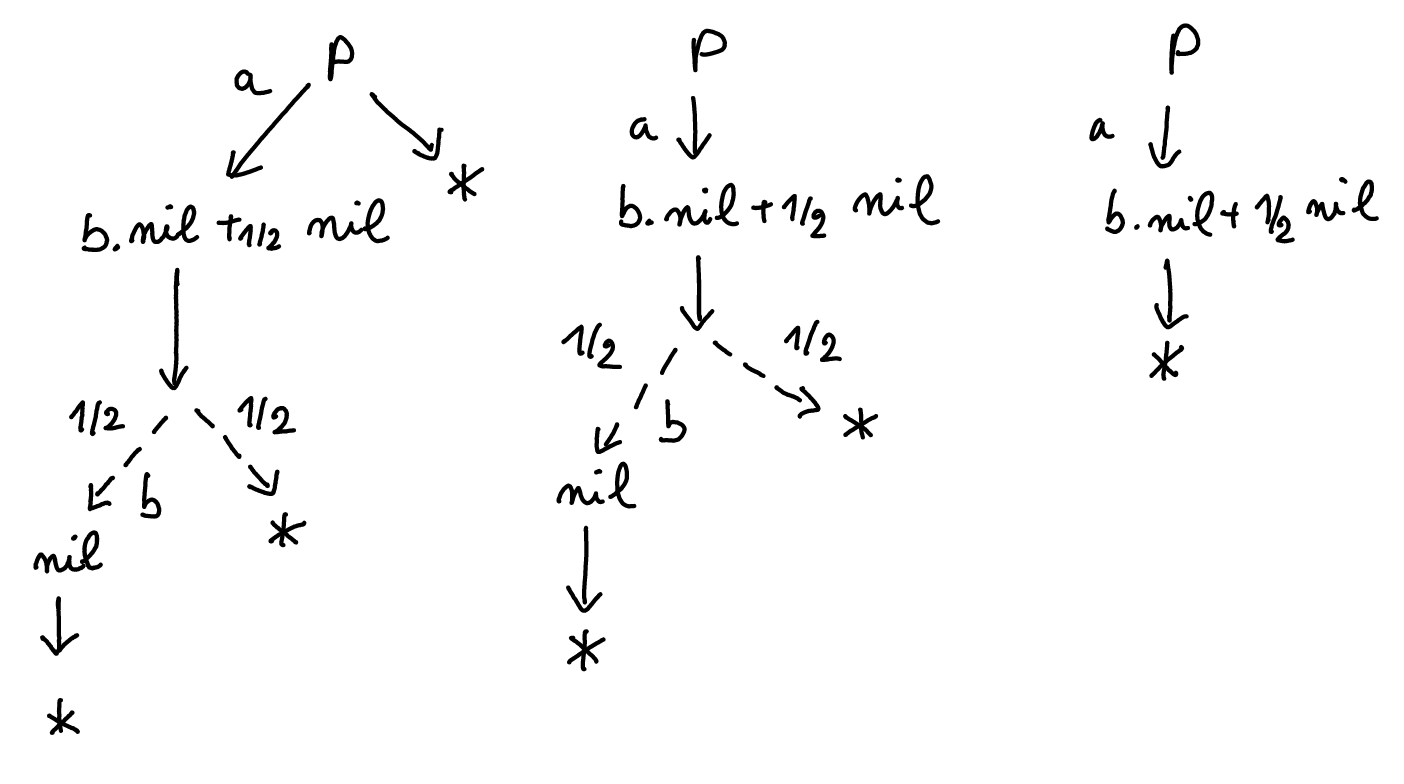
\includegraphics[width=\linewidth]{traces2.png}

\end{frame}

\begin{frame}{A Behavioral Equivalence}
    \begin{block}{Behavioral Equivalence (a kind of bisimulation)}
    \begin{itemize}
        \item $Set$-endofunctor $F$ 
        \item coalgebra $c : X \to FX$
        \item equivalence relation $R \subseteq X \times X$ 
        \item $q: X \to X/R$ the quotient map
    \end{itemize}
    $R$ is a \textbf{behavioral equivalence} if $(F(q) \circ c )(x) = (F(q) \circ c )(y)$ for all $(x,y) \in R$.  
    \end{block}
   
    \pause
    
    \begin{block}{Behaviorally equivalent elements}
        \begin{itemize}
        \item $Set$-endofunctor $F$ 
        \item coalgebra $c : X \to FX$
        \end{itemize}
        $x,y \in X$ are \textbf{behaviorally equivalent} ($x \simeq_F y$) if there exists a behavioral equivalence $R$ such that $(x,y) \in R$.
    \end{block}
    
\end{frame}

\begin{frame}{Behavioral Equivalence for Processes}
        
    \begin{example}
        For $F = \C + 1$, this is the known %convex
        bisimulation equivalence of Segala.
    \end{example}

    How to compute it in practice in our case? \pause Using the continuations and the presentations!

    \begin{example}[ $P_2 = a^2.\operatorname{\overline{\star}}$
  and $ P_3 = a.(a.\operatorname{\overline{\star}} \overline \oplus \operatorname{\overline{\star}})$
   ]
    For every semantics above, $\tau(P_1) = a.\operatorname{\overline{\star}}$, $\tau^2(P_1) = \operatorname{\overline{\star}}$  and $ \tau(P_3) = a.\operatorname{\overline{\star}} \oplus \operatorname{\overline{\star}}$. With the bottom axiom,  $$\tau^2(P_3) = \tau(a.\operatorname{\overline{\star}}) \oplus \tau(\operatorname{\overline{\star}}) = \operatorname{\overline{\star}} \oplus \star \overset{(\bot)}{=} \operatorname{\overline{\star}} .$$
    \end{example}

     \pause

    \begin{theorem}[Soundness and completeness]
        $P \simeq_F Q$ iff the equation $\tau^n(P) = \tau^n(Q)$ is derivable for some $n\in \mathbb N$ using the equations $E$ of a presentation $(\Sigma, E)$ of $F$.
    \end{theorem}

\end{frame}

\begin{frame}{Summing up}
\pause
    \begin{itemize}
        \item Algebraic presentation as a tool: \pause reasoning about systems algebraically, syntax that can give us intuition about how the semantics work \pause
        \item We saw the theory that presents $\C(+1)$ and $(+1)\C$ \pause but also the monad represented by the theory $\Th^{\star}_{CS} \cup \bot$
        \pause
        \item Soundness and completeness 
    \end{itemize}
\end{frame}

\begin{frame}{Looking ahead (blog post)}
\pause
    \begin{itemize}
        \item Switch from the concept of \textit{program equivalence} to that of \textit{program distance}
        \pause
        \item There exists a lifting $\hat \C \colon \cat{Met} \to \cat{Met}$
        \pause
        \item For $(X,d)$ a metric space, with distance function $d \colon X \times X \to \mathbb{R}$, we endow $\C(X)$ with a metric $HK(d)$: Hausdorff–Kantorovich
        \pause
        \item Question: how to lift with termination?
        \pause
        \item We will see that $\C(+1)$ and $\C^{\downarrow}$ can be lifted with the Hausdorff–Kantorovich metric, but there is no monad structure for lifting $(+1)\C$ with this metric
        \pause
        \item We will also see presentations via quantitative equational theories
    \end{itemize}
\end{frame}

\begin{frame}
    \begin{center}
        Thank you!
    \end{center}
\end{frame}

\end{document}